\documentclass{article}
\usepackage[utf8]{inputenc}
\usepackage{graphicx}
\usepackage{tikz}
\usepackage{lipsum} % Paquete para generar texto de relleno
\usepackage{fancyhdr} % Paquete para encabezados y pies de página
\usepackage[left=3cm, right=3cm, top=2.5cm, bottom=2.5cm]{geometry} % Paquete para ajustar los márgenes
\usepackage{tocloft} % Para personalizar el índice
\usepackage{parskip} % Para añadir espacios entre párrafos
\usepackage{minted}
\usepackage{xcolor} % Paquete para usar colores
\usepackage{grffile}
\usepackage{natbib} % Paquete para estilo de citas
\usepackage{tabularx}

%Definitions
\definecolor{lightgray}{gray}{0.5}

\renewcommand{\contentsname}{Índice}
\renewcommand{\cfttoctitlefont}{\hfill\Large\bfseries}
\renewcommand{\cftsecleader}{\cftdotfill{\cftdotsep}} % Rellena con puntos las secciones
\renewcommand{\cftsubsecleader}{\cftdotfill{\cftdotsep}} % Rellena con puntos las subsecciones
\renewcommand{\cftaftertoctitle}{\par\noindent\hrulefill\par\nobreak\vskip -0.5\baselineskip}

\newcommand{\horasVhdl}[2]{\textbf{Horas invertidas en el diseño de VHDL:} Iván D.: #1, Víctor M.P: #2\par\nointerlineskip}
\newcommand{\horasEntenderEnunciado}[2]{\textbf{Horas invertidas en entender el enunciado proporcionado:} Iván D.: #1, Víctor M.P: #2\par\nointerlineskip}
\newcommand{\horasDepuracion}[2]{\textbf{Horas invertidas en depurar el proyecto en busca de fallos:} Iván D.: #1, Víctor M.P: #2\par\nointerlineskip}
\newcommand{\horasMemoria}[2]{\textbf{Horas invertidas en el desarrollo de la memoria del proyecto:} Iván D.: #1, Víctor M.P: #2\par\nointerlineskip}

\fancypagestyle{plain}{
    \fancyhf{}
    \renewcommand{\headrulewidth}{0pt} % Elimina la línea de encabezado
    \fancyfoot[R]{\thepage} % Número de página a la derecha
}

% Configuración del encabezado y pie de página
\pagestyle{fancy}
\fancyhf{} % Limpia los encabezados y pies de página predeterminados
\renewcommand{\footrulewidth}{0.4pt}
\fancyfoot[L]{\textit{AOC - Proyecto 2}} % Encabezado izquierdo con el título del proyecto
\fancyhead[L]{\textit{Iván Deza, Víctor Martínez}}
\fancyfoot[R]{\thepage} % Pie de página centrado con el número de página
\renewcommand{\footrule}{\hbox to\headwidth{\color{lightgray}\leaders\hrule height \headrulewidth\hfill}}
\renewcommand{\headrule}{\hbox to\headwidth{\color{lightgray}\leaders\hrule height \headrulewidth\hfill}}


\begin{document}

\begin{titlepage}
    \centering
    \vspace*{\fill}
    \begin{figure}[htbp]
        \centering
        \begin{tikzpicture}[remember picture ,overlay]
          \node[opacity=0.1,inner sep=0pt, rotate=30] at (0, -6) {
\includegraphics[width=0.90\paperwidth]{assets/unizar.png}}; % Cambia "tu_logo.png" por el nombre de tu archivo de imagen del logo
        \end{tikzpicture}
    \end{figure}
    \vspace*{\fill}
    
    {\scshape\LARGE Universidad de Zaragoza \par}
    \vspace{0.5cm}
    \rule{\linewidth}{0.5mm} % Línea horizontal
    \vspace{0.5cm}
    {\scshape\Large Departamento de Organización de Computadoras \par}
    \vspace{0.5cm}
    \rule{\linewidth}{0.5mm} % Línea horizontal
    \vspace{1.5cm}
    {\huge\bfseries AOC - Proyecto 2\par}
    \vspace{0.5cm}
    {\Large\itshape Jerarquía de Memoria \par}
    \vspace{2cm}
    {\Large\itshape Iván Deza y Víctor Martinez \par}
    \vspace{0.5cm}
    {\Large\itshape José L. Briz, Javier Resano y Alejandro Valero \par}
    \vfill
    % Agrega la fecha si lo deseas
    {\large \today\par}
\end{titlepage}

\newpage

\tableofcontents

\newpage
\section{Introducción}
El proyecto en cuestión trata de el diseño e implementación de una unidad de control que sea capaz de controlar una jerarquía de memoria
donde tenemos: una memoria cache, de rápido acceso, una memoria Scratch de datos, también de acceso rápido, además de una memoria principal más lenta que las anteriores mencionadas.
Esta jerarquía de memoria viene conectada vía un bus, de tipo semisincrono, que actúa de árbitro entre todas las memorias de la jerarquía. Además la política de funcionamiento de la cache es \textbf{Fetch on Write Miss} (traemos el bloque que necesitamos cuando hay un fallo de escritura)
y \textbf{Copy Back} (no actualizamos escrituras a la memoria principal instantaneamente si no cuando hay un fallo y nos deshacemos de ese bloque). \par
Esta jerarquía de memoria se introduce en el chip MIPS del proyecto número 1, al cual se le ha cambiado el MD subsystem por uno más complejo, el cual incluye una jerarquía de memoria.\par
Además de esto, en el apartado 8.1, hemos comentado como funciona un ataque de canal lateral a una memoria cache, demostrado su funcionamiento y creado una prueba de concepto para este tipo de ataques. Tambien se propone una estrategia para mitigar esta vulnerabilidad.

\section{Diagrama de Estados de la UC}
\lipsum[1-3] % Texto de relleno

\section{Descomposición de Dirección}
\lipsum[4-6] % Texto de relleno

\section{Análisis de Latencias}
\lipsum[6-8] %texto de relleno
\subsection{Ciclos Efectivos}
\lipsum[9-10]

\section{Programas de Prueba}
\lipsum[10-12]

\section{Ejemplo de Código}
\lipsum[13-14]

\section{Apartados Opcionales}
\subsection{Hacking Ético}
En este apartado hemos querido enseñar como podíamos realizar un ataque DOS (denial of service o denegación de servicio), si sabemos como esta estructurada la memoria cache de un procesador.\par
Para detectarlo, podríamos usar un contrador de Write Missess, y que si ese valor es igual o muy cercano al numero de writes que se esta haciendo, saltar una señal alertando que posiblemente este tipo de ataque esta tendiendo lugar. 
Para solucionar esto lo que podríamos hacer es implementar un bit de lock, de manera que ciertas instrucciones que podamos marcar, no abandonarían nunca la cache. Mejorando el rendimiento del procesador frente a este tipo de ataques. Otra solución podría ser mandar un 
halt de manera que terminaríamos este proceso (en caso de que la cpu sea uniciclo). 
Información sobre este tipo de ataque: \cite{BackCache}.

\newpage

\section{Horas Dedicadas}

\begin{table}[h]
\centering
\begin{tabularx}{\textwidth}{|X|}
\hline
\horasDepuracion{0}{0} \\
\hline
\horasEntenderEnunciado{1}{0} \\
\hline
\horasMemoria{0}{0} \\
\hline
\horasVhdl{1}{0} \\
\hline
\end{tabularx}
\end{table}

\section{Autoevaluación}
\lipsum[15-18]

\newpage
\section{Anexo}
\subsection{Imágenes}
\begin{figure}[htbp]
  \centering
  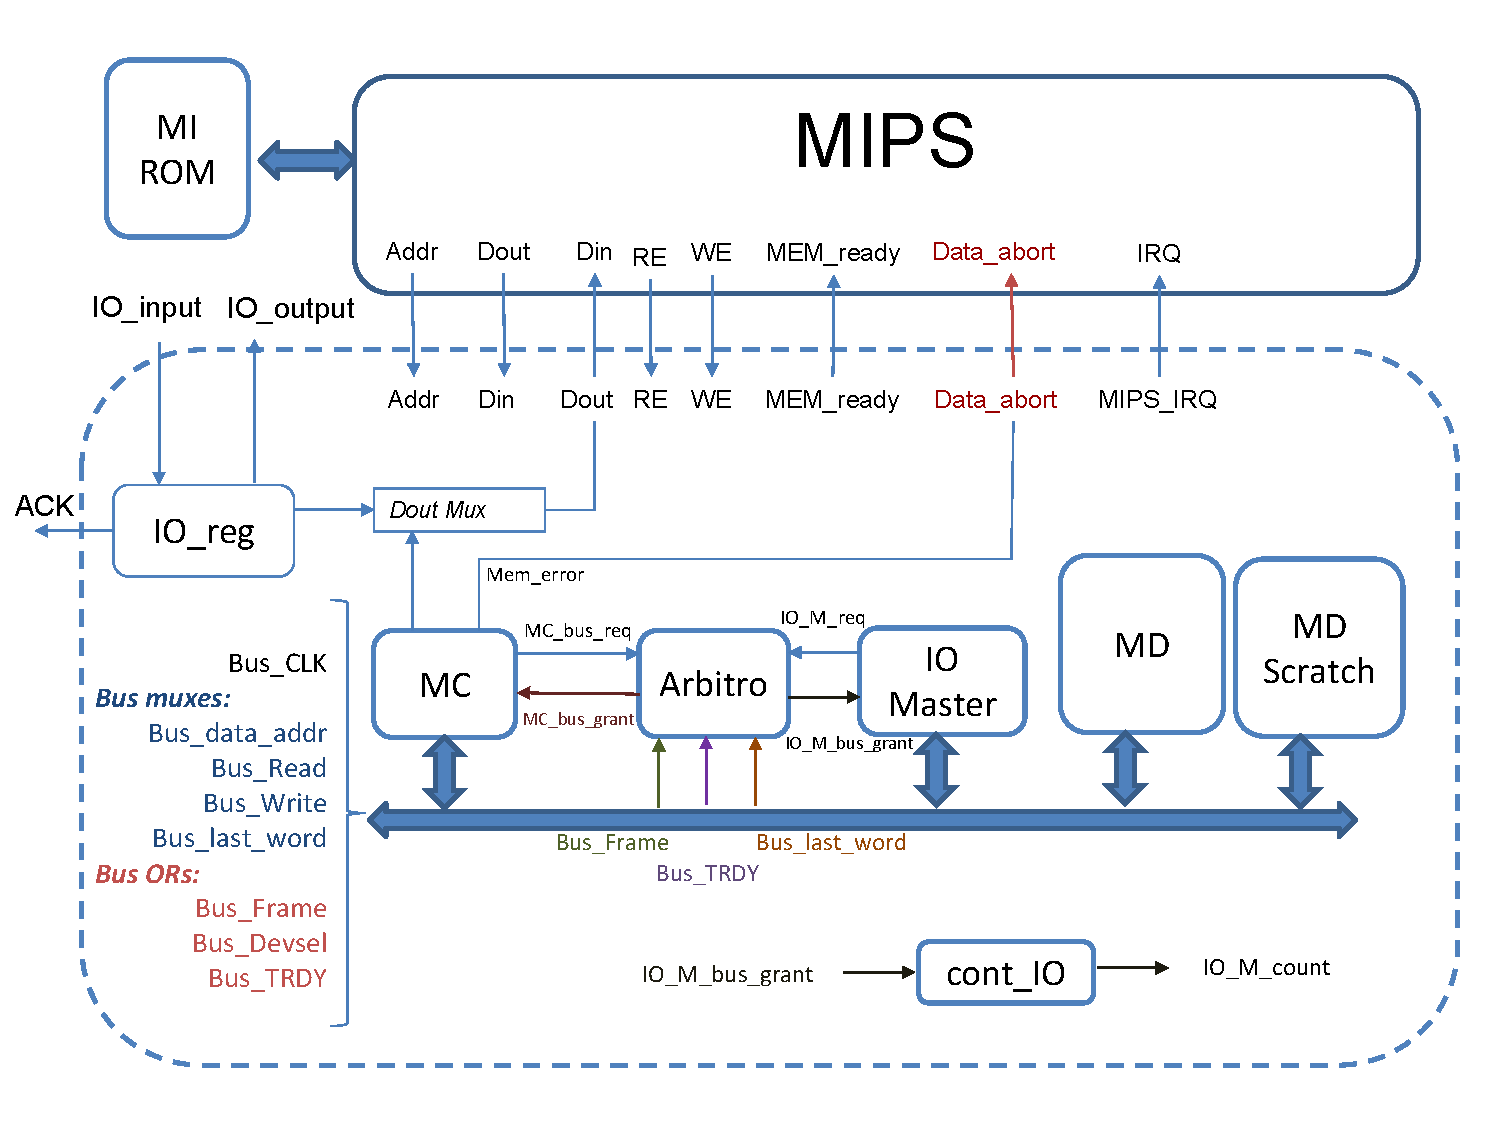
\includegraphics[page=1, width=0.8\textwidth, clip]{assets/AOC2_2024_Esquemas_Proy2.pdf}
  \caption{Esquema y señales principales del nuevo IO MD subsytem y de su bus. Se pide dise˜nar la
Unidad de Control de la MC}
  \label{fig:imagen}
\end{figure}

\newpage
\bibliographystyle{apalike}
\bibliography{assets/biblio} % Enlaza al archivo de bibliografía sin la extensión .bib



\end{document}

